% Template:     Auxiliar LaTeX
% Documento:    Archivo principal
% Versión:      8.3.3 (20/01/2025)
% Codificación: UTF-8
%
% Autor: Pablo Pizarro R.
%        pablo@ppizarror.com
%
% Manual template: [https://latex.ppizarror.com/auxiliares]
% Licencia MIT:    [https://opensource.org/licenses/MIT]

% CREACIÓN DEL DOCUMENTO
\documentclass[
	spanish, % Idioma: spanish, english, etc.
	letterpaper, oneside
]{article}

% INFORMACIÓN DEL DOCUMENTO
\def\documenttitle {Auxiliar 4}
\def\documentsubject {Dinámica}

\def\documentauthor {Nombre del autor}
\def\coursename {Mecánica}
\def\coursecode {FI-2001}

\def\universityname {Universidad de Chile}
\def\universityfaculty {Facultad de Ciencias Físicas y Matemáticas}
\def\universitydepartment {Departamento de la Física}
\def\universitydepartmentimage {departamentos/fcfm}
\def\universitydepartmentimagecfg {height=1.75cm}
\def\universitylocation {Santiago de Chile}

% EQUIPO DOCENTE
\def\teachingstaff {
	\textbf{Profesor: Claudia Scóccola} \\
	Auxiliares: Jorge Barja, Clemente Miranda, Matías Zúñiga \\
	Ayudante: Mario Calderón  \\
}

% IMPORTACIÓN DEL TEMPLATE
\input{template}

% INICIO DE PÁGINAS
\begin{document}

% CONFIGURACIÓN DE PÁGINA Y ENCABEZADOS
\templatePagecfg

% ======================= INICIO DEL DOCUMENTO =======================

% \newboxquestion{P1}\\

% Considere una bolita de masa $m$ ensartada en una barra de manera que puede deslizar sin roce por ella. La masa está atada mediante un resorte, de constante elástica $k$ y largo natural $l_0$, a un extremo de la barra, y esta última, a su vez, gira c/r al mismo extremo en un plano horizontal con velocidad angular $w$ constante. En $t=0$ la bolita se suelta con resorte comprimido en $l_0/2$ y $\dot{\rho}(0) = 0$:

% \begin{enumerate}[label=\alph*)]
%     \item ¿Qué relación deben cumplir $m,k$ y $w$ para que la bolita realice un movimiento armónico simple a lo largo de la barra?.
%     \item Determine la compresión del resorte como función del tiempo..

% \end{enumerate}


% \begin{figure}[ht] % [h] indica que se coloca la imagen aquí (here)
%     \centering % Centra la imagen
%     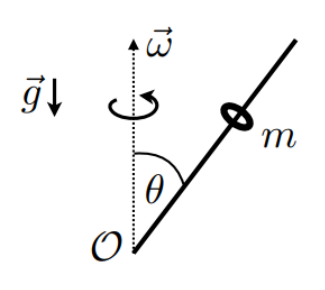
\includegraphics[width=0.4\textwidth]{p1.png} % Ajusta el tamaño de la imagen
%     \caption{Pregunta 1.} % Subtítulo de la imagen
%     \label{fig:p1} % Etiqueta opcional para referencias
% \end{figure}

\newboxquestion{P1}\\

Una argolla de masa $m$ puede deslizar sin roce a lo largo de una varilla que gira con
velocidad angular uniforme $\dot\phi = w_0 $, siempre formando un ángulo $\theta$ constante con la vertical.

\begin{enumerate}[label=\alph*)]

    \item  Usando una fuerza normal de la forma $\vec N = N_\theta \hat \theta + N_\phi \hat \phi$ , escriba la segunda ley de Newton, y encuentre la ecuación de movimiento que determina la distancia $r$ de la argolla al origen de la varilla $O$.

    \item Determine la solución de $r(t)$, para ello considere que en el tiempo inicial $r(t=0) = R$ y $\dot{r}(t=0) = 0$.

\end{enumerate}

% \begin{enumerate}[label=\alph*)]
%     \item Determine la forma de la fuerza de gravedad que actúa sobre $m$.
    
%     \item Usando una fuerza normal de la forma $\vec N = N_\theta \hat \theta + N_\phi \hat \phi$ , escriba la segunda ley de Newton, y encuentre la ecuación de movimiento que determina la distancia $r$ de la argolla al origen de la varilla $O$.
    
% \end{enumerate}


\begin{figure}[h]
    \centering
    \begin{subfigure}{0.48\textwidth}
        \centering
        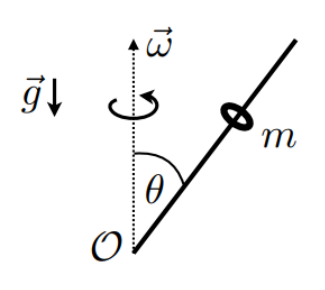
\includegraphics[width= 0.6\textwidth]{p1.png}
        \caption{Pregunta 1}
        \label{fig:p3}
    \end{subfigure}
    \hfill
    \begin{subfigure}{0.48\textwidth}
        \centering
        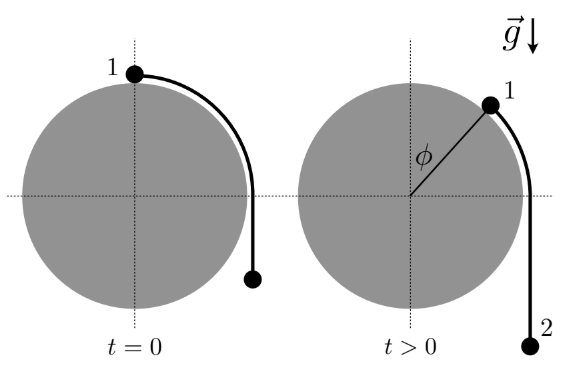
\includegraphics[width= 0.8\textwidth]{p3.png}
        \caption{Pregunta 2}
        \label{fig:p4}
    \end{subfigure}
    \label{fig:preguntas1}
\end{figure}




% \begin{figure}[ht] % [h] indica que se coloca la imagen aquí (here)
%     \centering % Centra la imagen
%     \hspace{-1.5cm} % Desplaza la imagen 2 cm a la izquierda
%     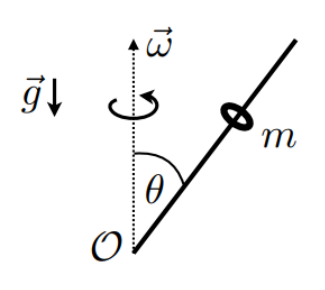
\includegraphics[width=0.3\textwidth]{p1.png} % Ajusta el tamaño de la imagen
%     \caption{Pregunta 1.} % Subtítulo de la imagen
%     \label{fig:p1} % Etiqueta opcional para referencias
% \end{figure}

\newboxquestion{P2} \\

Una partícula de masa $m$ (partícula 1) puede deslizar sin roce sobre la superficie de un cilindro de radio $R$. Una segunda partícula de igual masa (partícula 2) permanece atada a 1 mediante una cuerda ideal de largo $L > \pi R/2$. Inicialmente ($t = 0$) las partículas están en reposo, con 1 en la parte más alta del cilindro (ver figura).


\begin{enumerate}[label=\alph*)]
    \item Obtenga las ecuaciones de movimiento.
    \item Encuentre una ecuación que dependa solo de $\phi,\ddot{\phi}$.
    \item Integre la ecuación obtenida en la parte (b) para obtener $\dot \phi$ en función de $\phi$. 
    \item Obtenga una ecuación que permita determinar el ángulo en el cual la partícula 1 se despega del cilindro.

\end{enumerate}

% \begin{figure}[ht] % [h] indica que se coloca la imagen aquí (here)
%     \centering % Centra la imagen
%     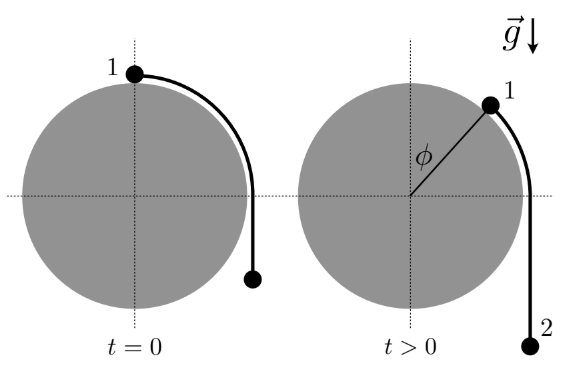
\includegraphics[width=0.4\textwidth]{p3.png} % Ajusta el tamaño de la imagen
%     \caption{Pregunta 2.} % Subtítulo de la imagen
%     \label{fig:p3} % Etiqueta opcional para referencias
% \end{figure}

% Una partícula de masa $m$ puede deslizar sin roce por el interior de una circunferencia de radio $R$ y eje horizontal. Se suelta desde la posición más baja, $\theta (0) = 0$, con velocidad angular $\dot{\theta}(0) = w_0$. Los datos son: $m$, $R$, $g$ y $w_0$.

% \begin{enumerate}[label=\alph*)]
%     \item Escriba la ecuación de movimiento (2da ley) y sepárela en ecuaciones escalares. Una de estas ecuaciones puede ser integrada una vez en forma inmediata.
  
%     \item Integrando tal ecuación se obtiene $\dot \theta ^2 = \textit{algo que tiene que ser positivo} $. Obtenga una desigualdad para $cos (\theta)$. ¿Físicamente qué ocurriría si la desigualdad se hiciera igualdad?.
  
%     \item Encuentre una expresión para la fuerza normal en función de los datos y de $\theta(t)$. Imponiendo que la fuerza normal apunte hacia el centro obtenga una desigualdad para $cos(\theta)$.¿Físicamente qué podría ocurrir si la desigualdad se hiciera igualdad?.

%     \item ¿Para qué valor de $w_0$ ambas desigualdades coinciden?.

%     \item Si el dibujo representa a una partícula que desliza apoyada en el interior de un cilindro de eje horizontal, ¿bajo qué condiciones la partícula oscila respecto al punto más bajo sin despegarse jamás?

%     \item ¿Bajo qué condiciones desliza girando en un solo sentido sin despegarse jamás?
% \end{enumerate}

% \begin{figure}[ht] % [h] indica que se coloca la imagen aquí (here)
%     \centering % Centra la imagen
%     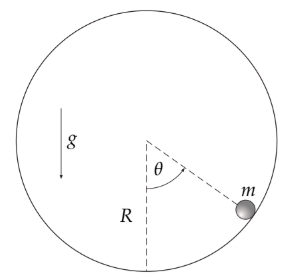
\includegraphics[width=0.3\textwidth]{p2.png} % Ajusta el tamaño de la imagen
%     \caption{Pregunta 2.} % Subtítulo de la imagen
%     \label{fig:p2} % Etiqueta opcional para referencias
% \end{figure}



\newboxquestion{P3}\\

Hay un hilo enrollado alrededor de un cilindro de radio $R$. En la punta del hilo hay un cuerpo de masa $m$ que se suelta,cuando $\phi =0$, con velocidad inicial $\vec{v}(t=0)=-v_0\hat{\rho}$, perpendicular al hilo, lo que determina que el hilo se comienza a enrollar. La distancia inicial entre el cuerpo y el punto $B$ de tangencia del hilo con el cilindro es $L_0$. \textbf{No hay gravedad.}

\noindent \textbf{Nota:} Las coordenadas cilíndricas en este problema persiguen al punto de tangencia $B$, y es conveniente escribir el vector posición como: $\vec{r} = R\hat{\rho} + L(t)\hat{\phi}$.

\begin{enumerate}[label=\alph*)]
    \item Determine la ecuación de movimiento para la distancia $L(t)$ correspondiente a la longitud de hilo que queda por enrollar en el tiempo $t$ (distancia entre los puntos $B$ y la posición de la masa).
    \item Obtenga la velocidad angular $\dot{\phi}$ en función de $\phi$.
    \item Suponiendo que el hilo se corta si la tensión sobrepasa el valor $T_{max}$, obtenga el valor de $\phi$ en el momento del corte (propuesto).
\end{enumerate}

\begin{figure}[ht]
    \centering
    % Primera imagen
    \begin{subfigure}[b]{0.24\textwidth}
        \centering
        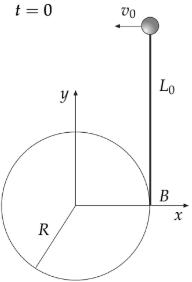
\includegraphics[width=\textwidth]{p4a.png}
        %\caption{Subtítulo de la segunda imagen}
        \label{fig:imagen1}
    \end{subfigure}
    \hspace{1.0 cm} % Espacio entre las imágenes
    % Segunda imagen
    \begin{subfigure}[b]{0.24\textwidth}
        \centering
        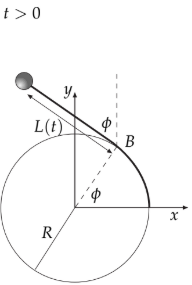
\includegraphics[width=\textwidth]{p4b.png}
        %\caption{Subtítulo de la segunda imagen}
        \label{fig:imagen2}
    \end{subfigure}
    \caption{Pregunta 3.}
    \label{fig:imagenes}
\end{figure}

\newpage

\newboxquestion{P4} \textbf{(Propuesto)}\\


Dos partículas, de masas $m_1$ y $m_2$, que están unidas por una cuerda de largo $d$, se mueven sin roce por el interior de un tubo. El tubo está unido de manera perpendicular a un eje que gira con velocidad angular constante $\Omega$. Inicialmente se suelta al sistema con movimiento nulo con respecto al tubo y con la masa $m_1$ a una distancia $R$ del eje.

\begin{enumerate}[label=\alph*)]
    \item Escriba las ecuaciones de movimiento y sepárelas en ecuaciones escalares.
  
    \item Resuelva estas ecuaciones y encuentre las distancias de las partículas al eje, $ρ_1$ y $ρ_2$, como funciones explícitas del tiempo.\\
    Sol: $\rho_1(t) = (R + \frac{m_2}{m_1 + m_2})cosh(\Omega t) - \frac{m_2}{m_1 + m_2}d \space ; \space \rho_2(t) = \rho_1(t) + d$ 
  
    \item Calcule el valor de la tensión de la cuerda.\\
    Sol: $T = \frac{m_1 m_2 d}{m_1^2 + m_2^2}\Omega ^2$

\end{enumerate}

\begin{figure}[ht] % [h] indica que se coloca la imagen aquí (here)
    \centering % Centra la imagen
    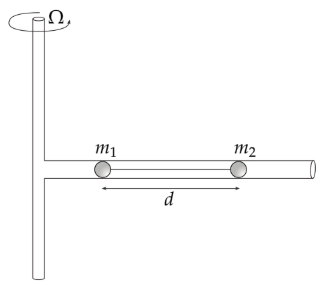
\includegraphics[width=0.25\textwidth]{p2_new.png} % Ajusta el tamaño de la imagen
    \caption{Pregunta 4.} % Subtítulo de la imagen
    \label{fig:p2} % Etiqueta opcional para referencias
\end{figure}



% FIN DEL DOCUMENTO
\end{document}